\documentclass{article}
\usepackage{algorithm2e}
\usepackage{algpseudocode}
\usepackage{graphicx}
\usepackage{subcaption}
\usepackage{float}
\graphicspath{{images/}}
\usepackage{amsmath}
\usepackage{amsthm}
\usepackage{amssymb}
\usepackage{dsfont}
\usepackage{hyperref}
\usepackage{xcolor}
\usepackage{ulem}
\usepackage[table]{xcolor}
\newcommand{\lemmaautorefname}{Lemma}
\newtheorem{corollary}{Corollary}
\newtheorem{theorem}{Definition}
\newtheorem{lemma}{Lemma}
\newtheorem{definition}{Definition}
\newtheorem{proposition}{Proposition}
\title{Alignment Problem for Tree-like Time Petri Nets}
\author{Ngoc Long Tran - Thomas Chatain}
\date{13 March 2025}



\begin{document}
\maketitle

\begin{abstract}
    Some results found during the research track, some notes and remarks.
\end{abstract}

\section{Tree-like Time Petri Net}
\begin{theorem}[Tree-like Time Petri Net]
    Let N = (P,T,F,SI,$\Sigma,\lambda,M_0,M_f$) be a Time Petri Net. N is Tree-like if it's connected, acyclic and \[\forall t \in T, |t^{\bullet}| \geq 1 \textit{ and } |{}^{\bullet}t| = 1,\] \[\forall p \in P, |p^{\bullet}| \leq 1 \textit{ and } |{}^{\bullet}p| \leq 1.\]
    N is so called Tree-like Time Petri Net.
\end{theorem}

\begin{figure}[h]
    \centering
    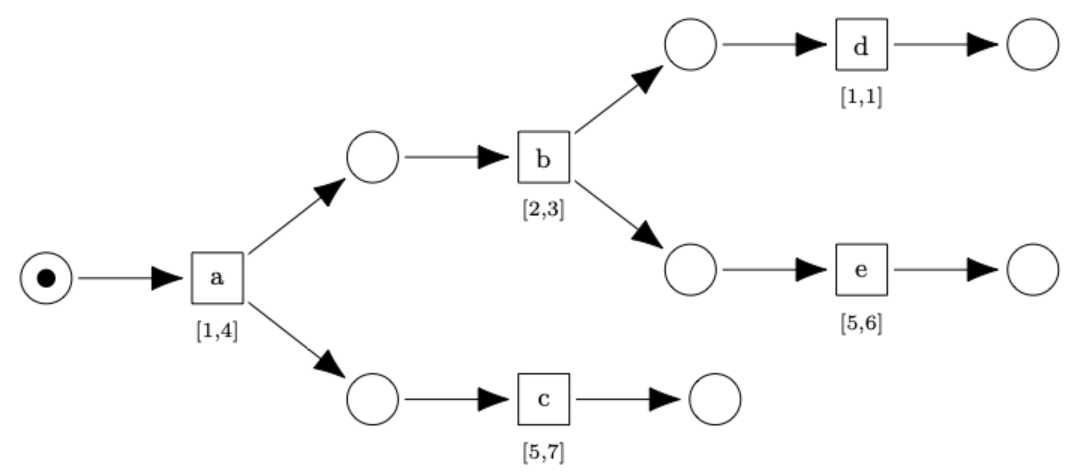
\includegraphics[width=0.75\linewidth]{images/Seq-Model 4.png}
    \caption{A Tree-like Time Petri Net}
\end{figure}

\section{Tree-like Time Petri Net : The alignment Problem}

The alignment problem in case of a model represented by a Tree-like Time Petri Net consists in measuring the deviation of a trace which is supposed to follow the model from the latter. Since the results depends strongly on the metric used to measure the deviation, we will focus on establishing here results for the Stamp Only Distance only. 
\vspace{0.3cm}

\textbf{Example:} Given a timed trace 
$\boldsymbol{\sigma} \text{ }\mathbf{= (a,3)(b,10)(c,4)(d,12)(e,15)}$ 
and a model represented by a Tree-like Time Petri Net shown above, 
we would like to align $\sigma$ with the Petri Net. In other words, 
what is the minimal cost to turn $\sigma$ into an accepted trace of the model ? 


\begin{figure}[h]
    \centering
    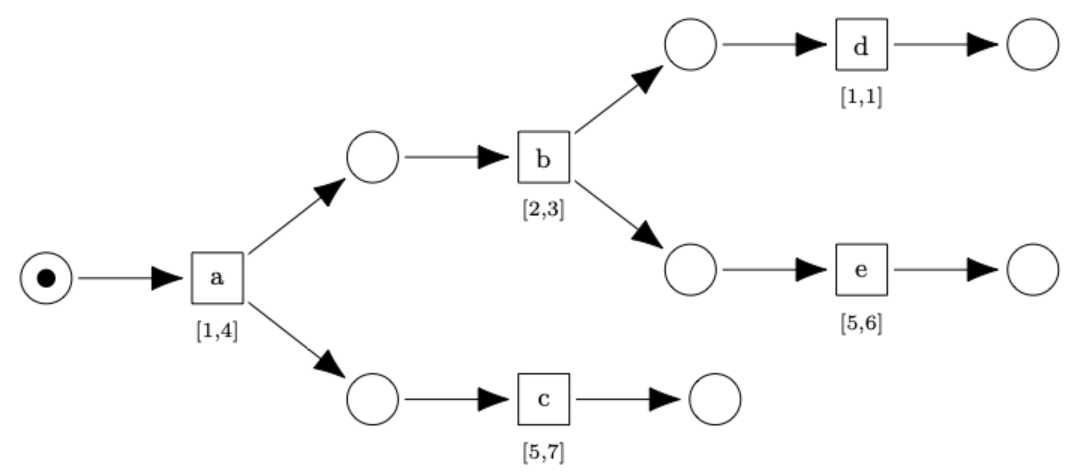
\includegraphics[width=0.75\linewidth]{images/Seq-Model 4.png}
    \caption{Model represented by a Tree-like Time Petri Net}
    \label{fig:Model represented by a Tree-like Time Petri Net}
\end{figure}

% \begin{itemize}
%     \item[$\blacksquare$]\uline{Greedy Approach} :
% \end{itemize}
Fistly, we can try to align the trace with the model in a greedy method by making the best decision
at each step and never turning back on decisions made. We start by aligning the root of the tree,
which is transition $a$. Since $a$ is executed at 3, which is between 1 and 4, we don't need to 
change its execution moment. 
\[\boldsymbol{\sigma_{aligned}} \text{ }\mathbf{= (a,3)...}\]
Then, we move to $a$'s children, which are $b$ and $c$.
$b$ must be fired between 2 and 3 after $a$, so the minimal cost of correcting $b$'s execution moment is 4,
by setting it to 6. Similarly, $c$ must be fired between 5 and 7 after $a$, so we set its execution moment to 8, 
which costs us 4. 
\[\boldsymbol{\sigma_{aligned}} \text{ }\mathbf{= (a,3)(b,6)(c,8)...}\]
Following the same reasoning, $d$ must be fired at 7 and $e$ at 12, which costs us 5 and 3 respectively.
\[\boldsymbol{\sigma_{aligned}} \text{ }\mathbf{= (a,3)(b,6)(c,8)(d,7)(e,12)}\]
The total cost of aligning $\sigma$ with the Petri net is 16. Now, let's try to get something 
better from $\boldsymbol{\sigma_{aligned}}$. 

\begin{tabular}{|c|c|c|c|c|c|}
    \hline
    Transition & a & b & c & d & e \\
    \hline
    Initial execution moment & 3 & 10 & 4 & 12 & 15 \\
    \hline
    Execution moment after greedy alignment & 3 & 6 & 8 & 7 & 12 \\
    \hline
    Modification & +0 & \textcolor{red}{-4} & +4 & \textcolor{red}{-5} & \textcolor{red}{-3} \\
    \hline
    Time constraints interval & [1,4] & [2,3] & [5,7] & [1,1] & [5,6] \\
    \hline
\end{tabular}

\vspace{0.3cm}
We notice that $a$ is initially executed at 3, which is in its time constraints interval [1,4]. So,
the best option at this level is not to change it. However, by doing so, node $b$ consequently needs to be shifted 
earlier and so are nodes $d$ and $e$ since they are standing on the left 
boundaries of the time constraints intervals. Thus, we had to make a lot of negative modifications
to align the trace with the model. Now if we change $a$'s execution moment to 4, it will cost us 1 
to modify  $a$'s execution moment but then $b$ can be set back to 7, $d$ to 8 and $e$ to 13, which reduces 
the cost by 3. Yet, this change will impact node $c$ by pushing its execution moment to 9, which means 
costing 1 more. Overall, we still manage to reduce the total cost by 1 and the new aligned trace is :
\[\boldsymbol{\sigma_{aligned}'} \text{ }\mathbf{= (a,4)(b,7)(c,9)(d,8)(e,13)}\]

This trace appears to be better than the previous one and it is also the best trace we can get that 
respects the time constraints of the model. The total cost of aligning $\sigma$ with the Petri net is 15.
In the following, we will give a systematic way to solve this problem and prove that the solution we found is indeed optimal.

% \begin{itemize}
%     \item[$\blacksquare$]\uline{Problem Analysis} :
% \end{itemize}

\subsection{Dynamic Programming Approach for the Alignment Problem}
Let's look at the model. We are interested in the execution moment of every transition and the places don't play any important role here. Thus, we will refer to every transition $i$ as \textit{\textbf{node}} and $i^{\bullet\bullet}$ or $\text{Child}(i)$ as set of its \textit{\textbf{children}}.
As shown in the model, time constraint between every node $i$ and $j \in \text{Child}(i)$ requires that $\sigma_{j} - \sigma_{i} \in [a_{j}, b_{j}]$. We also notice, in attempts to transform $\sigma$ into an accepted trace, that the order in which modifications are made has no impact on the distance between the initial trace and the final one. However, starting to align $\sigma$ with the Petri net by aligning the root of the tree results in changes in the execution moments of its children, and therefore poses once again the alignment problem for the subtrees. We recognize such similar substructures and thus try to tackle it with some recurrent equations.

% \begin{itemize}
%     \item[$\blacksquare$]\uline{Propositions} :
% \end{itemize}

\begin{theorem}[cost function]
    For all node $i$, considering the sub-tree of root ${}^\bullet i$ and the corresponding sub-sequence, by forgetting about $i$'s time contraints interval, let $d(i,x)$ be the minimal cost of setting the execution moment of node $i$ to $x$ and aligning the rest of the sub-tree with the sub-sequence, which is, in other words, adjusting the execution moments of $i$'s causal descendants so that the delays between each pair of two consecutive nodes fall within its time constraints interval in the sub-Petri net. 
\end{theorem}


As defined, $d(i,x)$ includes the cost of setting node $i$'s execution moment to $x$ which is $|\sigma_i - x|$. However, by changing the execution moment of node $i$ to $x$, $i$'s children might no longer respect their time constraints. Consequently, to align the sub-sequence with the sub-tree, $d(i,x)$ also needs to include the costs of correcting $i$'s children and their descendants, which are nothing else but $d(j,x_j)$ where $j \in \text{Child}(i)$ and $x_j$ is $j$'s new fixed execution moment. We then have: 

\begin{proposition}
    \begin{equation}
        \begin{split}
            d(i,x) & = |\sigma_{i}-x| + \min\Biggl\{\sum_{\substack{j \in \text{Child}(i) \\ x_{j}-x\in[a_{j},b_{j}]}}d(j,x_{j})\Biggr\} \\
            & = |\sigma_{i}-x| + \min\Biggl\{\sum_{\substack{j \in \text{Child}(i) \\ x_{j}\in[x+a_{j},x+b_{j}]}}d(j,x_{j})\Biggr\}
        \end{split}
    \end{equation}
\end{proposition}

In this case, the execution moment of each node $j$ must remain within the valid range $[x+a_{j}, x+b_{j}]$ and because $d(i,x)$ is the minimal cost of aligning the subsequence, $(x_{j})_{j \in \text{Child}(i)}$ must be chosen to minimize the sum. However, there are no constraints between children, each $x_{j}$ can be chosen independently to minimize the total cost:

\begin{proposition}
    \begin{equation}
        \begin{split}
            d(i,x) & = |\sigma_{i}-x| + \min\Biggl\{\sum_{\substack{j \in \text{Child}(i) \\ x_{j}\in[x+a_{j},x+b_{j}]}}d(j,x_{j})\Biggr\} \\
            & = |\sigma_{i}-x| + \sum_{j \in \text{Child}(i)}\min_{x_{j}\in[x+a_{j},x+b_{j}]}\{d(j,x_{j})\}\\
        \end{split}
    \end{equation}
\end{proposition}

% \begin{itemize}
%     \item[$\blacksquare$]\uline{Solution} :
% \end{itemize}


Now, suppose that $i$ is the root of the tree like Petri net and we get access 
to each value of $d(i,x)$ as $x$ varies. Then, the minimal cost of aligning the 
initial sequence with the Petri net is $\min_{x\in[a_i,b_i]}\{d(i,x)\}$, which 
is exactly the least cost to set the root's execution moment to a value between
$a_{root}$ and $b_{root}$ and aligning all its decendants to the Petri net.

\begin{proposition}
    The minimal cost of aligning the sequence with the whole Petri net 
    is \[\min_{x\in[a_{root},b_{root}]}\{d(root,x)\}\]. 
\end{proposition}

We are now interested in the nature of the function $d(i,\cdot)$ to be able to compute it effectively. 
The two following results give us some key properties of these functions.

\begin{lemma} 
    For any node $i$ of the tree, the function $d(i,\cdot)$ is a continuous, convex, 
    piecewise linear, and diverges to $+\infty$ at $\pm\infty$.
\end{lemma}

\begin{proof}
    We show by induction the property : For every node $u$ of the 
    tree, $H_i: d(i,\cdot) \text{ is a continuous, convex, piecewise linear function 
    which tends to } +\infty \text{ at } \pm\infty.$
    Initially, if $i$ is a leaf, $H_i$ is true directly since 
    $d(leaf,x) = |\sigma_{leaf} - x|$ is an absolute value function. 
    We climb up the tree and suppose that for every 
    $j \in \text{Child}(i)$, $H_j$ is true. The two first points above show that
    \begin{equation}
        \begin{split}
            d(i,x) & = |\sigma_{i}-x| + \sum_{j \in \text{Child}(i)}\min_{x_{j}\in[x+a_{j},x+b_{j}]}d(j,x_{j}) \\
            & = |\sigma_{i}-x| + \sum_{j \in \text{Child}(i)}g_j(x)
        \end{split}
    \end{equation}
    where $g_j : x\mapsto \min_{x_{j}\in[x+a_{j},x+b_{j}]}d(j,x_{j})$. 
    By induction hypothesis, $d(j,\cdot)$ is a continuous, convex, piecewise linear function 
    which tends to $+\infty$ at $+\infty$ and $-\infty$. According to 
    Lemma~\ref{lem:important} shown further below, $g_j$ also possesses these same properties. 
    Finally, since the sum of continuous, convex, piecewise linear functions 
    which tend to $+\infty$ at $+\infty$ and $-\infty$ is also a 
    function of the same type, 
    we deduce that $d(i,\cdot)$ also possesses these properties. Hence, the result.
\end{proof}

\begin{corollary} 
    Let d a continuous, convex, piecewise linear function whose limits 
    at $+\infty$ and $-\infty$ exist and are $+\infty$. There exist then $x_{0}$ and 
    $x_{1}$ such that $f$ decreases in $]-\infty,x_{0}]$, constant in $[x_{0},x_{1}]$ 
    and increases in $[x_{1},+\infty[$. We refer to these as decreasing, stationary and 
    increasing zones. As a consequence, every function $d(x,\cdot)$ possesses these 
    proprieties.
\end{corollary}
\subsubsection{Illustration on an example}

Let's illustrate the recurrence relation by solving the example above. 
We aim to align the sequence $\boldsymbol{\sigma} \text{ }\mathbf{= (a,3)(b,10)(c,4)(d,12)(e,15)}$  
with the Petri net shown in Figure~\ref{fig:Model represented by a Tree-like Time Petri Net}.



We start with the leaves. The cost of assigning a leaf with the value $x$ and its 
causal descendants with the subnet is $d(leaf,x) = |x-\sigma_{leaf}|$ only 
because a leaf doesn't have any children. We obtain the graphs of these functions 
\ref{fig:Cost function for leaves}. 

\begin{figure}[H]
    \centering
    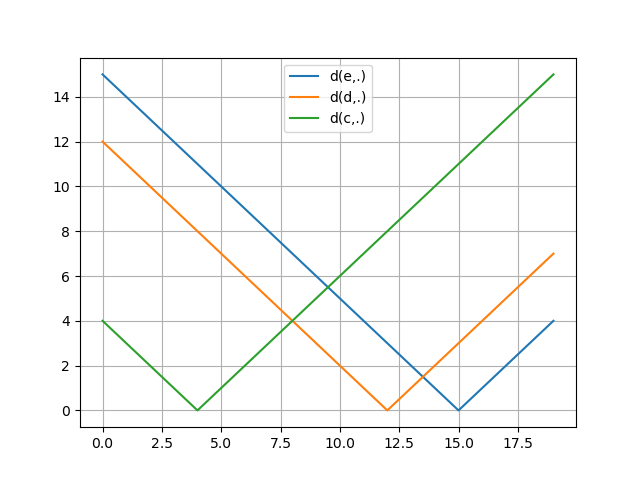
\includegraphics[width=0.85\textwidth]{images/d(feuille).png}
    \caption{Cost function for some leaves}
    \label{fig:Cost function for leaves}
\end{figure}

We continue by moving up the tree. For node $b$:
\begin{equation}
    \begin{split}
        d(b,x) & = |x-\sigma_b| + \sum_{j\in \text{Child}(b)}\min_{x_j \in [a_j+x,b_j+x]}d(j,x_j) \\
        & = |x-10| + \min_{x_d \in [1+x,1+x]}d(d,x_d) + \min_{x_e \in [5+x,6+x]}d(e,x_e) \\
    \end{split}
\end{equation}
Now, the calculations of $d(b,x)$ depend strongly on how we calculate the two last terms of 
the sum, since $|x-10|$ can be easily evaluated. We remarks that these two terms are of form 
$\min_{x_{node} \in [x+a,x+b]}d(node,x_{node})$. As $x$ increases, the segment $[x+a,x+b]$ 
progressively shifts from left to right, and we wish to calculate the minimum of 
$d(node,x_{node})$ over this segment.

% \begin{lemma} 
%     For any node $x$ of the tree, the function $d(x,\cdot)$ is a continuous, convex, 
%     piecewise linear, and diverges to $+\infty$ in $\pm\infty$.
% \end{lemma}

% \begin{corollary} 
%     Let d a continuous, convex, piecewise linear function whose limits 
%     at $+\infty$ and $-\infty$ exist and are $+\infty$. There exist then $x_{0}$ and 
%     $x_{1}$ such that $f$ decreases in $]-\infty,x_{0}]$, constant in $[x_{0},x_{1}]$ 
%     and increases in $[x_{1},+\infty[$. We refer to these as decreasing, stationary and 
%     increasing zones. As a consequence, every function $d(x,\cdot)$ possesses these 
%     proprieties.
% \end{corollary}

\begin{lemma} \label{lem:important} 
    For all real couple a,b s.t a $\leqslant$ b, and for all continuous, convex, 
    piecewise linear function f which tends to $+\infty$ at $+\infty$ and 
    $-\infty$, \[ g : x\mapsto \min_{t\in[x+a, x+b]}f(t) \] is also a continuous, 
    convex, piecewise linear function having $+\infty$ as limit at $\pm\infty$.
\end{lemma}

\begin{proof}
    We present here a method for obtaining the graph of $g$ from the graph of $f$. A rigorous proof can then be easily deduced. 

    Now, since $f$ is continuous, convex, piecewise linear, Corollary 1 implies the existence of two real numbers $x_0$ and $x_1$ such that $f$ decreases in $]-\infty,x_0]$, constant in $[x_0,x_1]$, increasing in $[x_1,+\infty[$. Then, the minimum of $f$ in the interval $[x+a, x+b]$ that slides from left to right as $x$ increases can be estimated based on the relative position between $[x_0,x_1]$ and $[x+a, x+b]$. We distinguish three cases: 
    \begin{itemize}
        \item[$\blacksquare$] When the intersection $[x_0, x_1] \cap [x + a, x + b]$ is nonempty, we have
\[
g(x) = \min_{t \in [x + a, x + b]} f(t) = \min_{\mathbb{R}} f,
\]
    since the interval $[x + a, x + b]$ contains points where $f$ attains its global minimum. Therefore, the graph of $g$ over the interval $[x_0 - b, x_1 - a]$ is a horizontal segment at height $y = \min_{\mathbb{R}} f$. That is, the graph can be obtained by shifting the graph of $f$ restricted to $[x_0, x_1]$ left by $b$ units and extending it to the right by $(b - a)$ units.
    
    \item[$\blacksquare$] When $x + b \leq x_0$, the interval $[x + a, x + b]$ lies entirely to the left of $x_0$, and $f$ decreases in this interval. Hence,
    \[
g(x) = \min_{t \in [x + a, x + b]} f(t) = f(x + b).
\]
    The graph of $g$ in the interval $]-\infty, x_0 - b]$ is obtained by shifting the graph of $f$ restricted to $]-\infty, x_0]$ left by $b$ units.
        
    \item[$\blacksquare$] When $x_1 \leq x + a$, the interval $[x + a, x + b]$ lies entirely to the right of $x_1$, and $f$ increases in this interval. Hence,
\[
g(x) = \min_{t \in [x + a, x + b]} f(t) = f(x + a).
\]
    The graph of $g$ in the interval $[x_1 - a, +\infty[$ is obtained by shifting the graph of $f$ restricted to $[x_1, +\infty[$ left by $a$ units.
    \end{itemize}
    Finally, $g$ can be drawn correctly as shown in an example illustrated in Figure \ref{fig:Graph_g} below.
    \begin{figure}[H]
        \centering
        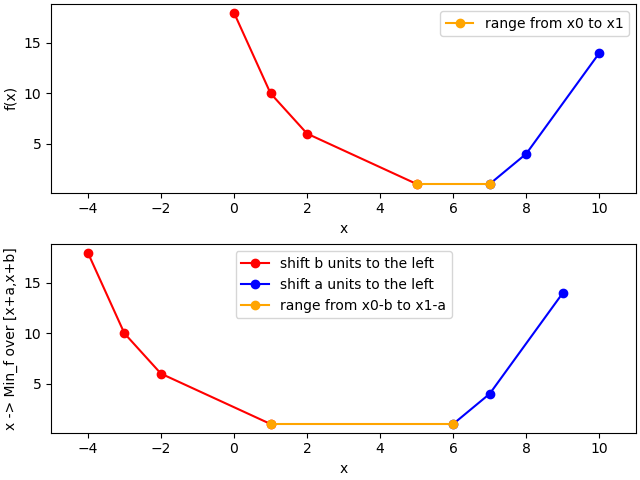
\includegraphics[width=1\linewidth]{images/translation.png}
        \caption{Example with $x_0$ = 5, $x_1$ = 7, a = 1, b = 4}
        \label{fig:Graph_g}
    \end{figure}
    Graphically, it is clear that $g$ is also a continuous, convex, piecewise linear function that has $+\infty$ as limit at $\pm\infty$. A rigorous proof can be driven by formalizing these arguments mentioned above and justifying the convexity of $g$ very easily.
\end{proof}
Returning to our example, we can now get access to the functions $x\mapsto \min_{x_d\in[x+1, x+1]}d(d,x_d)$ and $x\mapsto \min_{x_e\in[x+5, x+6]}d(e,x_e)$ \ref{fig:Leaf_d} \ref{fig:Leaf_e}.
\begin{figure}[H]
    \centering
    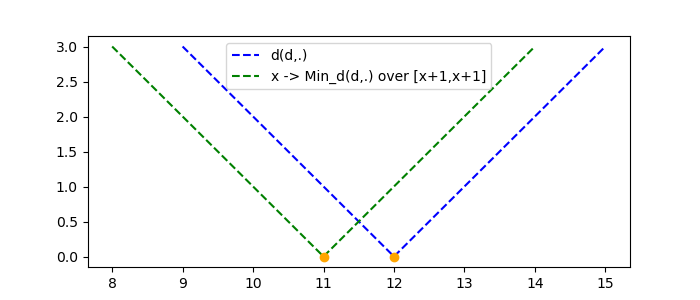
\includegraphics[width=\textwidth]{images/d_min(d).png}
    \caption{Leaf $d$}
    \label{fig:Leaf_d}
\end{figure}
\begin{figure}[H]
    \centering
    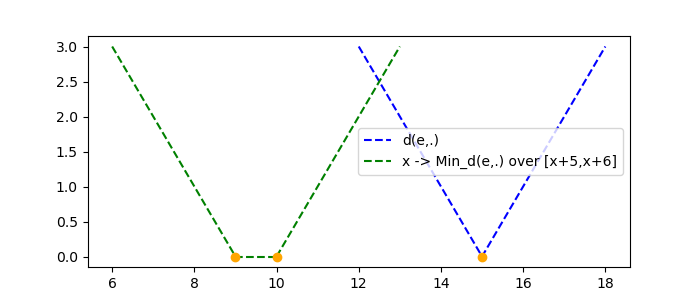
\includegraphics[width=\textwidth]{images/d_min(e).png}
    \caption{Leaf $e$}
    \label{fig:Leaf_e}
\end{figure}
Thus, computing \[d(b,x) = |x-10| + \min_{x_d \in [1+x,1+x]}d(d,x_d) + \min_{x_e \in [5+x,6+x]}d(e,x_e)\]  amounts to summing the contributions of 3 components, which can be read in graphs \ref{fig:Graph of d(b,.)}.
\begin{figure}[H]
    \centering
    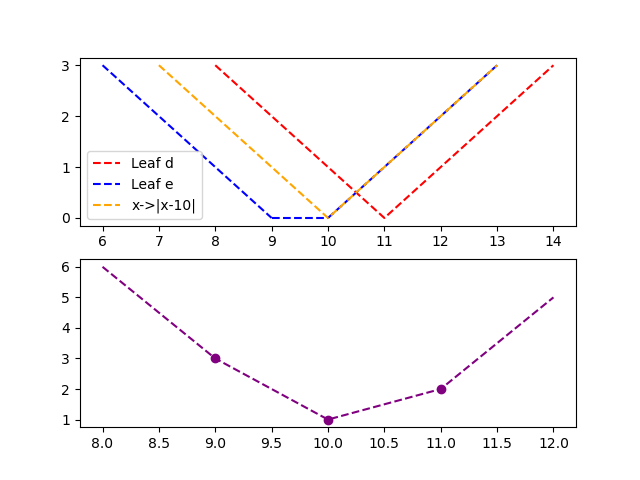
\includegraphics[width=1\linewidth]{images/d(b,x).png}
    \caption{Graph of $d(b,\cdot)$}
    \label{fig:Graph of d(b,.)}
\end{figure}
In this way, we are able to climb up the tree and to compute the function $d(a,\cdot)$ which answers to the question of minimal cost to align the sequence with the whole Petri net :
\begin{equation}
    \label{eq:5}
    \begin{split}
    d(a,x) & = |\sigma_a - x| + \min_{x_b\in[a_b+x,b_b+x]}d(b,x_b) + \min_{x_c\in[a_c+x,b_c+x]}d(c,x_c) \\
    & = |3 - x| + \min_{x_b\in[2+x,3+x]}d(b,x_b) + \min_{x_c\in[5+x,7+x]}d(c,x_c)
    \end{split}
\end{equation}
Finally, we obtain the cost function for the root \ref{fig:d(a,.)}. Zooming in a bit, we see that the graph attains its global minima on the interval $[6,7]$ but it is not the result directly. The first transition is fired between 1 and 4, the minimal cost of our alignment problem is \[\min_{x\in [1,4]}d(a,x)\] which is 15, attains at $x = 4$. 
Looking back to the equation \ref{eq:5}, we can deduce that the best alignment is obtained by setting $a$ to 4, then $b$ will be set to $x_{b}$ which minimizes $d(b,\cdot)$ over $[2+x,3+x]$. 
Since $x = 4$, $[2+x,3+x] = [6,7]$ and the minimum of $d(b,\cdot)$ over this interval is attained at 7. 
So $x_{b}$ is 7. Similarly, $x_{c}$ will be set to 9, $x_{d}$ to 8 and $x_{e}$ to 13. We then get the aligned trace 
\[\boldsymbol{\sigma_{aligned}'} \text{ }\mathbf{= (a,4)(b,7)(c,9)(d,8)(e,13)}\]
with a total cost of 15. This is exactly the result we found above.

\begin{figure}[H]
    \centering
    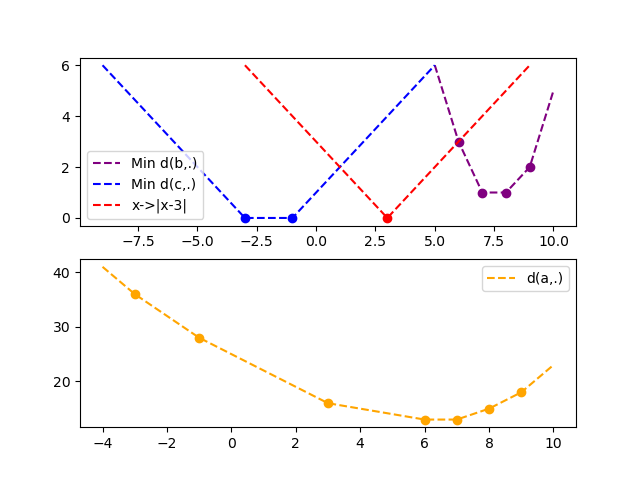
\includegraphics[width=1\linewidth]{d_a.png}
    \caption{Cost function $x\mapsto d(a,x)$}
    \label{fig:d(a,.)}
\end{figure}
\subsubsection{Complexity Analysis and Implementation}

In reality, a continuous, convex, piecewise linear function can be characterized by its leftmost and rightmost slopes and a set of points located at positions where the slopes changes. 
Also, by summing these functions, the sum is a function of the same type and its slopes change only at points where the slope of one of its components changes. 
Thus, it is possible to calculate an upper bound for the number of breakpoints of the functions $d(u,\cdot)$ for all node $u$.
\begin{lemma}
For a node $u$, let $S_{d(u,\cdot)}$ denote the set of breakpoints (points where slope changes) of the function $x \mapsto d(u,x)$, and $S_{\min d(u,\cdot)}$ for $x \mapsto \min_{x_u \in [a_u+x, b_u+x]} d(u,x_u)$. Then:
\begin{enumerate}
    \item $|S_{\min d(u,\cdot)}| \leq |S_{d(u,\cdot)}|+1 $
    \item $|S_{d(u,\cdot)}| = |\{\sigma_u\}\cup \bigcup_{j\in\text{Child}(u)}S_{\min d(u,\cdot)}|$
    \item $|S_{\min d(u,\cdot)}| \leq 2|T_u|$ where $T_u$ is the set of transitions of the subtree whose root is ${}^\bullet u$.
\end{enumerate}
\end{lemma}

\begin{proof}
    Scholium:
    \begin{enumerate}
        \item Based on the proof of \autoref{lem:important}, the graph of 
        $x\mapsto\min_{x_u \in [a_u+x,b_u+x]}d(u,x_u)$ can be obtained by 
        translating the graph of $x\mapsto d(u,x)$ and extending its stationary 
        zone. As a result, this extension of the stationary zone can at most add 
        one more point to $S_{\min d(u,\cdot)}$ compared to $S_{d(u,\cdot)}$.
        \item We know that 
        \[d(u,x) = |x-\sigma_u| + \sum_{j\in \text{Child}(u)}\min_{x_j \in [a_j+x,b_j+x]}d(j,x_j)\] 
        and by adding the affine functions, the slopes add up. Therefore, the sum, 
        which is also a piecewise linear function, can change its slopes only at 
        points where the slope of one of its components changes. Hence the result.
        \item We show by induction the property : For every node $u$ of the 
        tree, \[H_u: |S_{\min d(u,\cdot)}| \leq 2|T_u|.\] 
        Initially, if $u$ is a leaf, $H_u$ is true directly. 
        We climb up the tree and suppose that for every 
        $j \in \text{Child}(i)$, $H_j$ is true. The two first points above show that
        \begin{equation}
            \begin{split}
                |S_{\min d(u,\cdot)}| \leq 1 + |S_{d(u,\cdot)}| 
                & = 1 + |\{\sigma_u\}\cup \bigcup_{j\in\text{Child}(u)}S_{\min d(u,\cdot)}| \\
                & \leq 1 + |\{\sigma_u\}| + \sum_{j\in\text{Child}} |S_{\min d(u,\cdot)}| \\
                & \leq 2 + \sum_{j\in\text{Child}(u)}2|T_j|\\
                & = 2|T_u|
            \end{split}
        \end{equation}
        By deduction, the result is true for all nodes of the tree. Hence, the result. 
    \end{enumerate}
\end{proof}

Finally, we can sum up the algorithm within the following pseudo-code:

We implement the algorithm in Python and the code can be found \href{https://gitlab-student.centralesupelec.fr/ngoc-long.tran/parcours-recherche-time-aware-conformance-checking-and-model-repair/-/blob/9061323f09b85597fb2573d32ab0714499497fdb/modele_arborescent_stamp_only.py}{here}.
\begin{algorithm}[H]
    \caption{Aligning a timed trace with a Tree-like Time Petri Net under Stamp Only Distance}
    \SetAlgoLined
    \KwIn{A tree-like Time Petri Net N = (P,T,F,SI,$\Sigma,\lambda,M_0,M_f$) modelized by $G = (V,E)$ where 
    $V = T$ and $(t_i,t_j)\in E$ iff $t_j \in t_i^{\bullet\bullet}$ and a timed trace $\boldsymbol{\sigma} = (a_1,t_1)(a_2,t_2)...(a_n,t_n)$}
    \KwOut{The minimal cost of aligning $\boldsymbol{\sigma}$ with N and the aligned trace $\boldsymbol{\sigma_{aligned}}$}
    \SetKwProg{Fn}{Function}{:}{end}
    \Fn{Compute\_cost\_function($node$)}{
        \eIf{$node$ is a leaf}{
            \Return{$d(node,x) = |\sigma_{node} - x|$}\;
        }{
            $d(node,x) = |\sigma_{node} - x|$\;
            \ForEach{$child$ in Child($node$)}{
                $d(child,x) \gets$ Compute\_cost\_function($child$)\;
                $min\_d(child,x) \gets \min_{x_{child} \in [a_{child}+x,b_{child}+x]}d(child,x_{child})$\;
                $d(node,x) \gets d(node,x) + min\_d(child,x)$\;
            }
            \Return{$d(node,x)$}\;
        }
    }
    $optimal\_cost \gets$ Compute\_cost\_function($Root(G)$)\;
    $\boldsymbol{\sigma_{aligned}} \gets []$\; 
    $x_{parent,aligned} \gets 0$\;
    \Fn{Align\_trace($node$, $x_{parent,aligned}$)}{
        $x_{node, aligned} \gets argmin_{x_{node}-x_{parent,aligned} \in [a_{node},b_{node}]}d(node,x_{node})$\;
        \If{$node$ is a leaf}{
            \Return\;
        }
        \ForEach{$child$ in Child($node$)}{
            Align\_trace($child$, $x_{node, aligned}$)\;
        } 
    }
    \Return{$optimal\_cost, \boldsymbol{\sigma_{aligned}}$}\;
\end{algorithm}

The complexity of the algorithm mainly depends on the 
calculation of $d(node,x)$ for each node of the tree. For 
a node $u$, calculating $d(u,x)$ requires summing the 
contributions of its children, which can be done in 
$O(|\text{Child}(u)| \cdot |S_{d(j,\cdot)}|)$ time, where 
$j \in \text{Child}(u)$. Since $|S_{d(j,\cdot)}|$ is bounded 
by $2|T_j|$ according to the previous lemma, the time 
complexity for computing $d(u,x)$ becomes 
$O(|\text{Child}(u)| \cdot |T_j|)$. Summing this over 
all nodes in the tree, we find that the overall time 
complexity of the algorithm is $O(|T|^2)$, where $|T|$ 
is the number of transitions in the Petri net. This quadratic 
complexity arises from the need to compute and store the cost 
functions for each node and their children.

Function Align\_trace traverses the tree once, and at each node,
determines the optimal execution moment based on the precomputed cost functions 
in $O(1)$ time. In total, this function runs in $O(|T|)$ time and 
so the overall time complexity of the algorithm is
$O(|T|^2) + O(|T|) = O(|T|)^2$. 

\subsubsection{Testing and Results}

To show the performance of our algorithm, we test the code on randomly generated 
Tree-like Time Petri Nets of different sizes and measure the execution time. The 
results are plotted in the graph as following \ref{fig:Execution time of the algorithm on randomly generated Tree-like Time Petri Nets}. Note 
that the time constraints intervals are randomly generated in [1,10] and the timed trace is
chosen randomly so that the difference between two consecutive transitions is also in [1,10].
\begin{figure}[H]
    \centering
    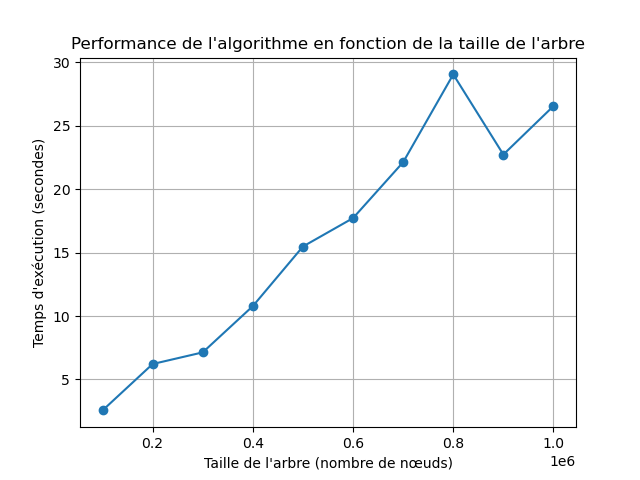
\includegraphics[width=0.75\linewidth]{images/Execution_time.png}
    \caption{Execution time of the algorithm on randomly generated Tree-like Time Petri Nets}
    \label{fig:Execution time of the algorithm on randomly generated Tree-like Time Petri Nets}
\end{figure}

\end{document}

